\documentclass{article}

% Language setting
% Replace `english' with e.g. `spanish' to change the document language
\usepackage[english]{babel}

% Set page size and margins
% Replace `letterpaper' with `a4paper' for UK/EU standard size
\usepackage[letterpaper,top=2cm,bottom=2cm,left=3cm,right=3cm,marginparwidth=1.75cm]{geometry}

% Useful packages
\usepackage{fancyhdr}
\usepackage{amsmath}
\usepackage{graphicx}
\usepackage[colorlinks=true, allcolors=blue]{hyperref}
\usepackage{titlesec}
\usepackage{enumitem}
\usepackage{amssymb}
\usepackage{amsthm}
\usepackage{tikz}
\usepackage{pgfplots}
\usepackage{float}
\usepackage{subcaption}
\usepackage{listings}
\usepackage{color}

\title{\vspace*{-3cm} % Adjusted to reduce the top margin
      \begin{center}
            \hspace*{0cm} % Adjusted to extend the black strip to the left
            \begin{tabular}{l@{}c@{}r}
                  \begin{tabular}{@{}c}
                        \textbf{Problem Chosen} \\
                        \textcolor{red}{\textbf{C}}
                  \end{tabular} &
                  \begin{tabular}{@{}c}
                      \textbf{2024} \\
                      \textbf{MCM/ICM} \\
                      \textbf{Summary Sheet}
                  \end{tabular} &
                  \begin{tabular}{@{}c}
                      \textcolor{black}{\textbf{Team control number}} \\
                      \textcolor{red}{\textbf{2417022}}
                  \end{tabular}
            \end{tabular} \\[0.3cm]
            \rule{\linewidth}{2pt} % Adjust the width and height here
            \vspace{-2.5cm} % Adjusted to reduce the bottom margin
      \end{center}
      \vspace{2cm}
      \textbf{\LARGE Uncover the secrets behind Alcaraz's success in Wimbledon}
}

\date{} % Removes the date
\author{} % Removes the author

\begin{document}
\maketitle
\begin{center}
      \Large\textbf{Abstract}
\end{center}
Abstract goes here.

% Define header and footer
\pagestyle{fancy}
\fancyhf{} % Clear default header and footer
% Header
\fancyhead[C]{\textbf{Tennis Model}} % Centered header content
\fancyhead[L]{\textit{Team control number 2417022}} % Left-aligned header content

% Footer
\fancyfoot[C]{\thepage} % Centered page number
\fancyfoot[L]{\textcolor{gray}{2024 MCM/ICM C 2417022}} % Left-aligned footer content
\fancyfoot[R]{\textcolor{gray}{}} % Right-aligned footer content

\newpage
\tableofcontents % Table of contents
\newpage

\section{Introduction}
\subsection{Background}
Tennis originated in the 13th century in France. As early as the 16th to 17th centuries, French missionaries often played a game similar to tennis in the corridors of churches, using their hands to strike a small ball,
providing a diversion from the monotonous church life. Now, modern tennis has formally developed and quickly gained popularity in Europe and America, becoming a widely loved sport. [1] Tennis, as a charming and elegant sport, enjoys a high reputation and strong influence internationally. [2] With the continuous development of tennis, the fluctuations in the scores of opponents have become increasingly scrutinized during tennis matches. Recently, in the men's singles final at Wimbledon in 2023, 20-year-old Spanish rising star Carlos Alcaraz defeated 36-year-old Novak Djokovic, ending Djokovic's winning streak at Wimbledon since 2013. The twists and turns in the score and the changing dynamics of the match attracted significant attention. Therefore, effectively exploring the impact of the "momentum" on the score during the game is crucial.

\subsection{Problem restatement}
\begin{enumerate}
\item  Develop a mathematical model to quantify and visualize the progression of tennis matches, identifying key performance metrics for players during specific time intervals, with a particular focus on the service advantage.
\item Construct a statistical framework to assess the impact of momentum within a match, challenging the notion that players' swings in performance are random, and providing empirical evidence for or against this assertion.
\item Formulate a predictive model capable of indicating potential shifts in match dynamics, utilizing data from previous matches to identify indicators that signal when the flow of play may change in favor of one player over another.
\item Execute a comprehensive testing protocol for the aforementioned models across a series of matches, evaluating the predictive capabilities with respect to different match conditions, and identifying additional variables that may enhance future model iterations. Analyze the generalizability of the models to other match formats and sporting contexts, such as women's tennis, various tournaments, court surfaces, and racket sports akin to table tennis.
\end{enumerate}
\subsection{Our Work}
Firstly, the choice of model should be grounded in the context of the problem, taking into account the importance of momentum in tennis matches and its impact on player performance. Therefore, the model needs to capture the dynamic changes during a match and reflect the performance of players at different points in time. Factors such as scoring probability, fatigue levels, technical skills, and the mental state during the match are crucial indicators of momentum change, so the chosen model should integrate these factors to predict the scoring probability of players. Given that the dataset provides detailed match scores and other relevant statistics, machine learning algorithms like LGBM and XGBOOST are suitable choices because they can handle a large number of features and are applicable to classification problems. Moreover, considering the sequential nature of scoring in tennis matches, time series analysis or Hidden Markov Models could be used to capture the momentum changes throughout the match.
Taking all these factors into account, opting for gradient boosting algorithms (such as LGBM or XGBOOST) for modeling is a wise decision. These algorithms perform well in dealing with complex relationships and nonlinear patterns and can manage large datasets efficiently. Additionally, incorporating sequence models to capture temporal momentum changes should also be considered. The final model selection will be based on predictive accuracy (metrics such as accuracy, recall, precision, F1 score, AUC, and ROC curves) and the model's interpretability. Such a model will be able to assess the impact of "momentum" on the probability of scoring for players and provide insights into the presence of non-random fluctuations in matches.
\section{Problem Analysis}
In the first study, multiple key factors affecting the scoring abilities of tennis players were comprehensively considered. This included not only whether they were serving but also factors like their level of fatigue, technical skills, and psychological state during the match. A comprehensive evaluation system was designed to deeply analyze these variables, such as individual technical levels, degrees of fatigue, and real-time mental states during matches. By employing statistical Logistic regression, the proposed system of indicators was tested for its correlation with players' scoring, and its effectiveness was validated on a dataset of tennis matches. Machine learning techniques, including LGBM, XGBOOST, support vector machines, perceptron networks, and logistic regression, were applied along with five-fold cross-validation and multi-dimensional performance metrics. The gradient boosting algorithm LGAM was ultimately chosen to dynamically assess players' real-time performance, or what is referred to as match "momentum."

The second study focused on exploring whether the "momentum" effect during matches has statistical significance, that is, whether the fluctuations in players' scoring during matches are non-random. The optimized machine learning model developed in the first study was applied to a test dataset, with predicted scoring probabilities compared to actual scoring records of athletes, and validated through Pearson correlation analysis. Subsequently, a univariate linear regression model was established, using predicted "momentum" as the independent variable and players' scoring as the dependent variable, to quantify the impact of "momentum" on scoring.

The third study addressed the challenges of model construction, as the model from the first study primarily focused on predicting the scoring probability of each serve and shot, rather than volatility prediction. To bridge this gap, the predictive focus was adjusted from individual shots to the outcome of entire games, analyzing fluctuations in players' performances across individual sets and the entire match. By aggregating features, a predictive model was built using statistical Logistic regression, with the support vector machine chosen as the final model. Model performance was evaluated using LGBM, XGBOOST, recall, precision, F1 score, AUC, and ROC curves. The information gain method was employed to determine the importance of various variables in the indicator system, leading to recommendations for athletes' future performance in matches.

In the final study, by selecting four matches as a validation set and using other match data as a training set, the visualization method of the ROC-AUC curve showcased the model's performance differences across various matches. Considering the uncertainty of the "volatility" indicator, machine learning evaluation standards were used for performance evaluation. In tests across these four matches, the constructed model demonstrated significant performance differences. Given this, expandable research directions were proposed, emphasizing the importance of individual athlete abilities and proving the applicability and strong generalizability of the proposed indicator system in other competitions


\section{Model Assumption}
\begin{enumerate}
\item The server has a greater advantage over the receiver.This assumption posits that the player initiating the serve in a game is more likely to gain an upper hand.
\item Players are affected by the "momentum" of the match.It's assumed that the success or failure of players during a match influences their future performance, suggesting that momentum plays a critical role in the outcome of the game.
\item A player's technical skill has a significant and direct impact on their scoring performance.This assumption highlights the importance of individual skills and how they translate into points on the board.
\item Fatigue affects players during the match, impacting their performance in the later stages.This suggests that as the match progresses, players' energy levels and their ability to maintain peak performance diminish.
\item The psychological state of players, including their ability to handle mistakes and respond to critical moments, significantly influences the match.This assumption underscores the importance of mental toughness and psychological preparedness in determining a player's success in competition.
\end{enumerate}
\section{Symbol Description}
\begin{table}[H]
\centering
\begin{tabular}{|c|l|}
\hline
\textbf{Symbol} & \textbf{Description} \\ \hline
$S1$ & The number of game winning in the current set \\ \hline
$S2$ & The leading scores in the current game \\ \hline
$S3$ & Whether it is the server \\ \hline
$S4$ & Whether score in the last point \\ \hline
$S5$ & The score lead progress of this match\\ \hline
$S6$ & Whether the serve is scored (no contact) \\ \hline
$S7$ & Whether to score on a return kick (no touch). \\ \hline
$S8$ & No touch score on the backhand \\ \hline
$S9$ & Is there a double fault in this game? \\ \hline
$S10$ & Whether there were unforced errors in this game. \\ \hline
$S11$ & The ratio of the number of times you use the Internet to the number of times you use the Internet. \\ \hline
$S12$ & The ratio of the chance of scoring when the opponent serves to the number of points actually scored. \\ \hline
$S13$ & Total mileage in this match \\ \hline
$S14$ & The total mileage in the last three points \\ \hline
$S15$ & Mileage chart from last point \\ \hline
$S16$ & Serve real-time pace \\ \hline
\end{tabular}
\caption{Symbol Description}
\end{table}
\section{Model Construction and Analysis}
\subsection{Task1's Model}
\subsubsection{Data Preprocessing}
In the initial phase of data preprocessing, the dataset is imported from a .csv file, and the Pandas library is employed to structure the data into a DataFrame. Subsequent to this, the dropna function is applied to eliminate records with missing values. Following the initial data preparation, the script undertakes a comprehensive feature engineering process, introducing novel features pertinent to the distinct characteristics of tennis matches.

In the subsequent phase, the dataset is readied for modeling through a meticulous iteration over each data point. This involves the extraction of features and the assignment of labels contingent upon the outcome of each point, specifically focusing on point victories. To enhance the robustness and suitability of the data for subsequent machine learning applications, the features undergo scaling. The MinMaxScaler from the scikit-learn library is employed for this purpose, ensuring that all variables are standardized within the [0, 1] range. This standardization is imperative to mitigate the undue influence of certain features during the modeling process, arising from variations in scale.

The finalization of the preprocessing sequence involves the preservation of the processed and standardized dataset in an Excel file. These methodical steps collectively address challenges associated with missing values, outliers, and standardization, culminating in the generation of a refined dataset poised for efficacious utilization in machine learning endeavors.
\subsubsection{Model Analysis}
The analysis of player performance in tennis is a multifaceted task that requires a comprehensive approach, blending traditional statistical methods with advanced machine learning techniques. In this section, we delve into the intricacies of our model, examining the preprocessing steps, model training, evaluation metrics, and the overall performance against various benchmarks.

Initially, we employed logistic regression to assess the statistical significance of the relationship between our established indicator system and the corresponding labels. Leveraging a tennis match dataset, we computed these indicators and labels indicating player scoring. This step not only aids in comprehending how various factors impact a player's score but also lays a crucial groundwork for feature selection in the modeling phase.

Subsequent to this, we utilized a range of machine learning algorithms, including LGBM, XGBoost, Support Vector Machines, Perceptron Networks, and Logistic Regression. We compared their effectiveness using metrics like accuracy, recall, precision, F1-score, AUC, and ROC curves. This step not only robustly supports our final choice of the LGAM algorithm for modeling but also ensures the model's capacity for generalization.

In the concluding phase, we opted for the LGAM algorithm for modeling. This algorithm not only dynamically evaluates a player's performance but also captures shifts in "momentum" during a match. This dynamic assessment model facilitates more accurate predictions of a player's performance, enhancing the precision of predicting match outcomes. Through this research, we have taken a noteworthy stride in comprehending and appraising player tactics and scoring, establishing a strong basis for more in-depth analysis and prediction.

Concerning the creation of the indicator system, we analyzed potential factors influencing a tennis player's scoring. The system was formulated based on elements like player fatigue, real-time and historical scoring situations, and the player's psychological state. This thorough analysis contributes to a nuanced understanding of player performance, paving the way for further exploration and prediction.
\begin{figure}[htbp]
      \centering
      \begin{subfigure}{0.48\textwidth} % Adjust the width as needed
          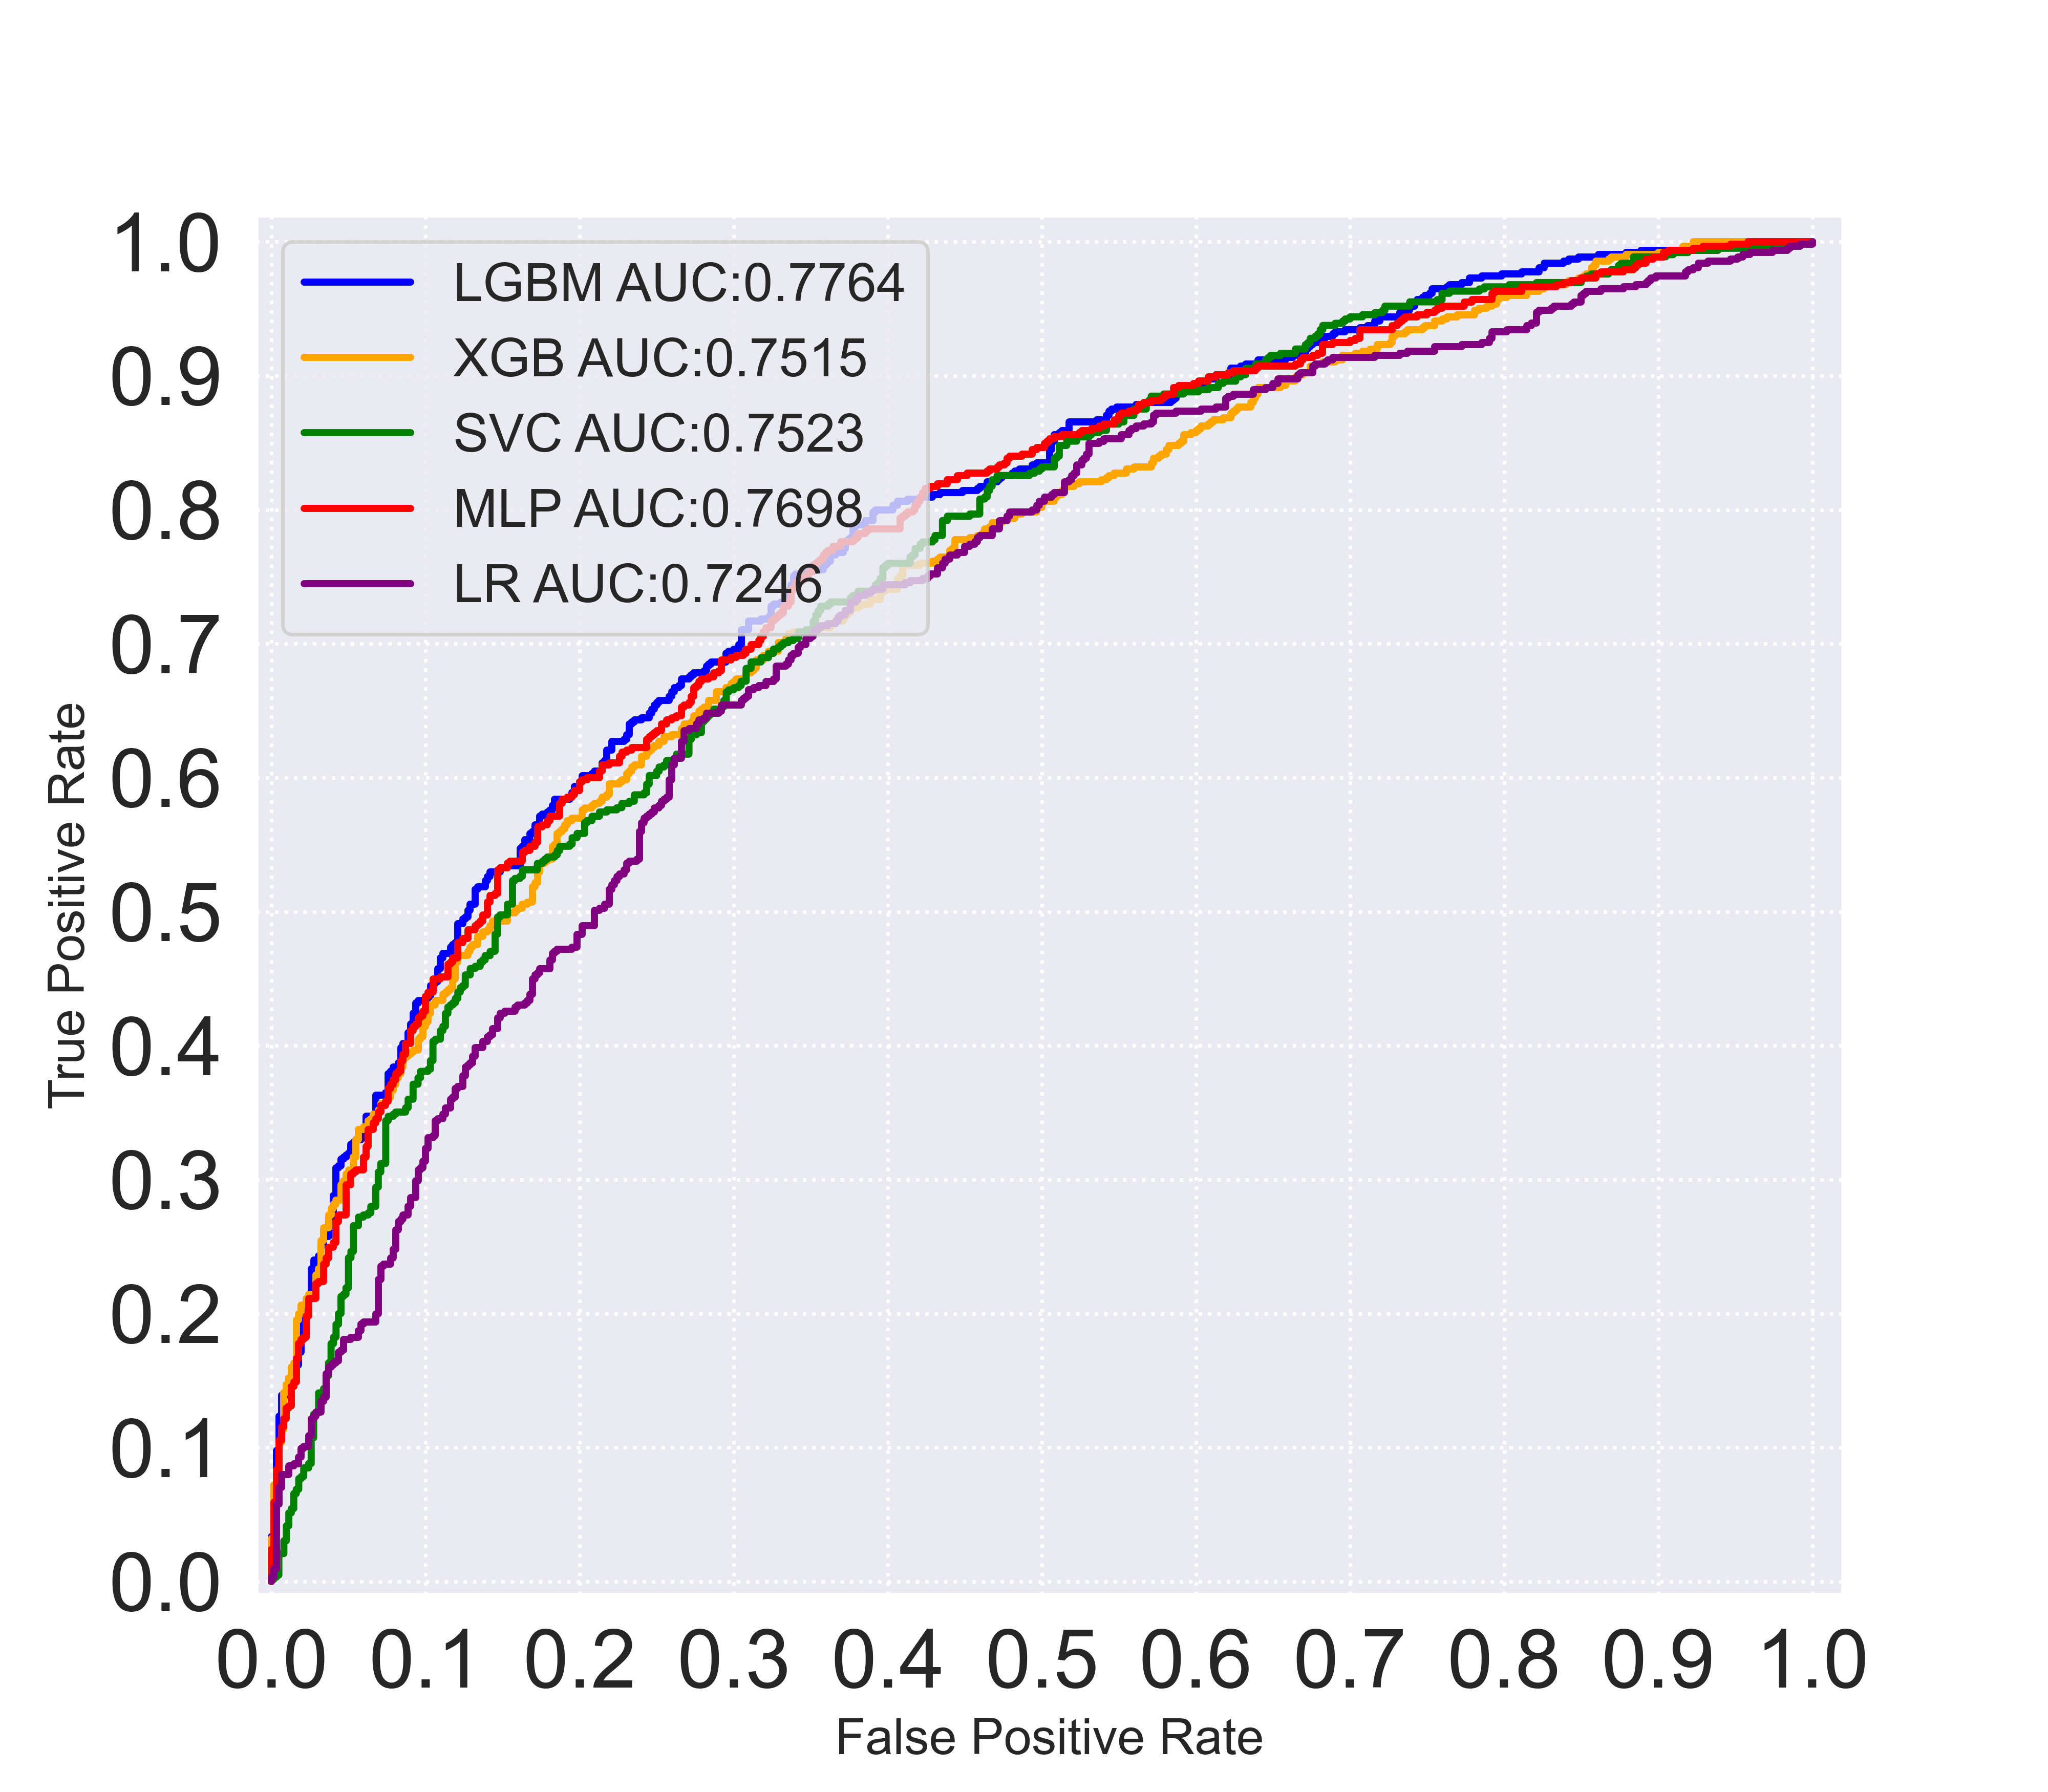
\includegraphics[width=\linewidth]{task1_image\roc_auc(test(before_sampling)).png} % Replace 'figure1' with the filename of your first figure
          \caption{roc_auc_test}
          \label{fig:roc_test}
      \end{subfigure}
      \hfill % Add horizontal space between the subfigures
      \begin{subfigure}{0.48\textwidth} % Adjust the width as needed
          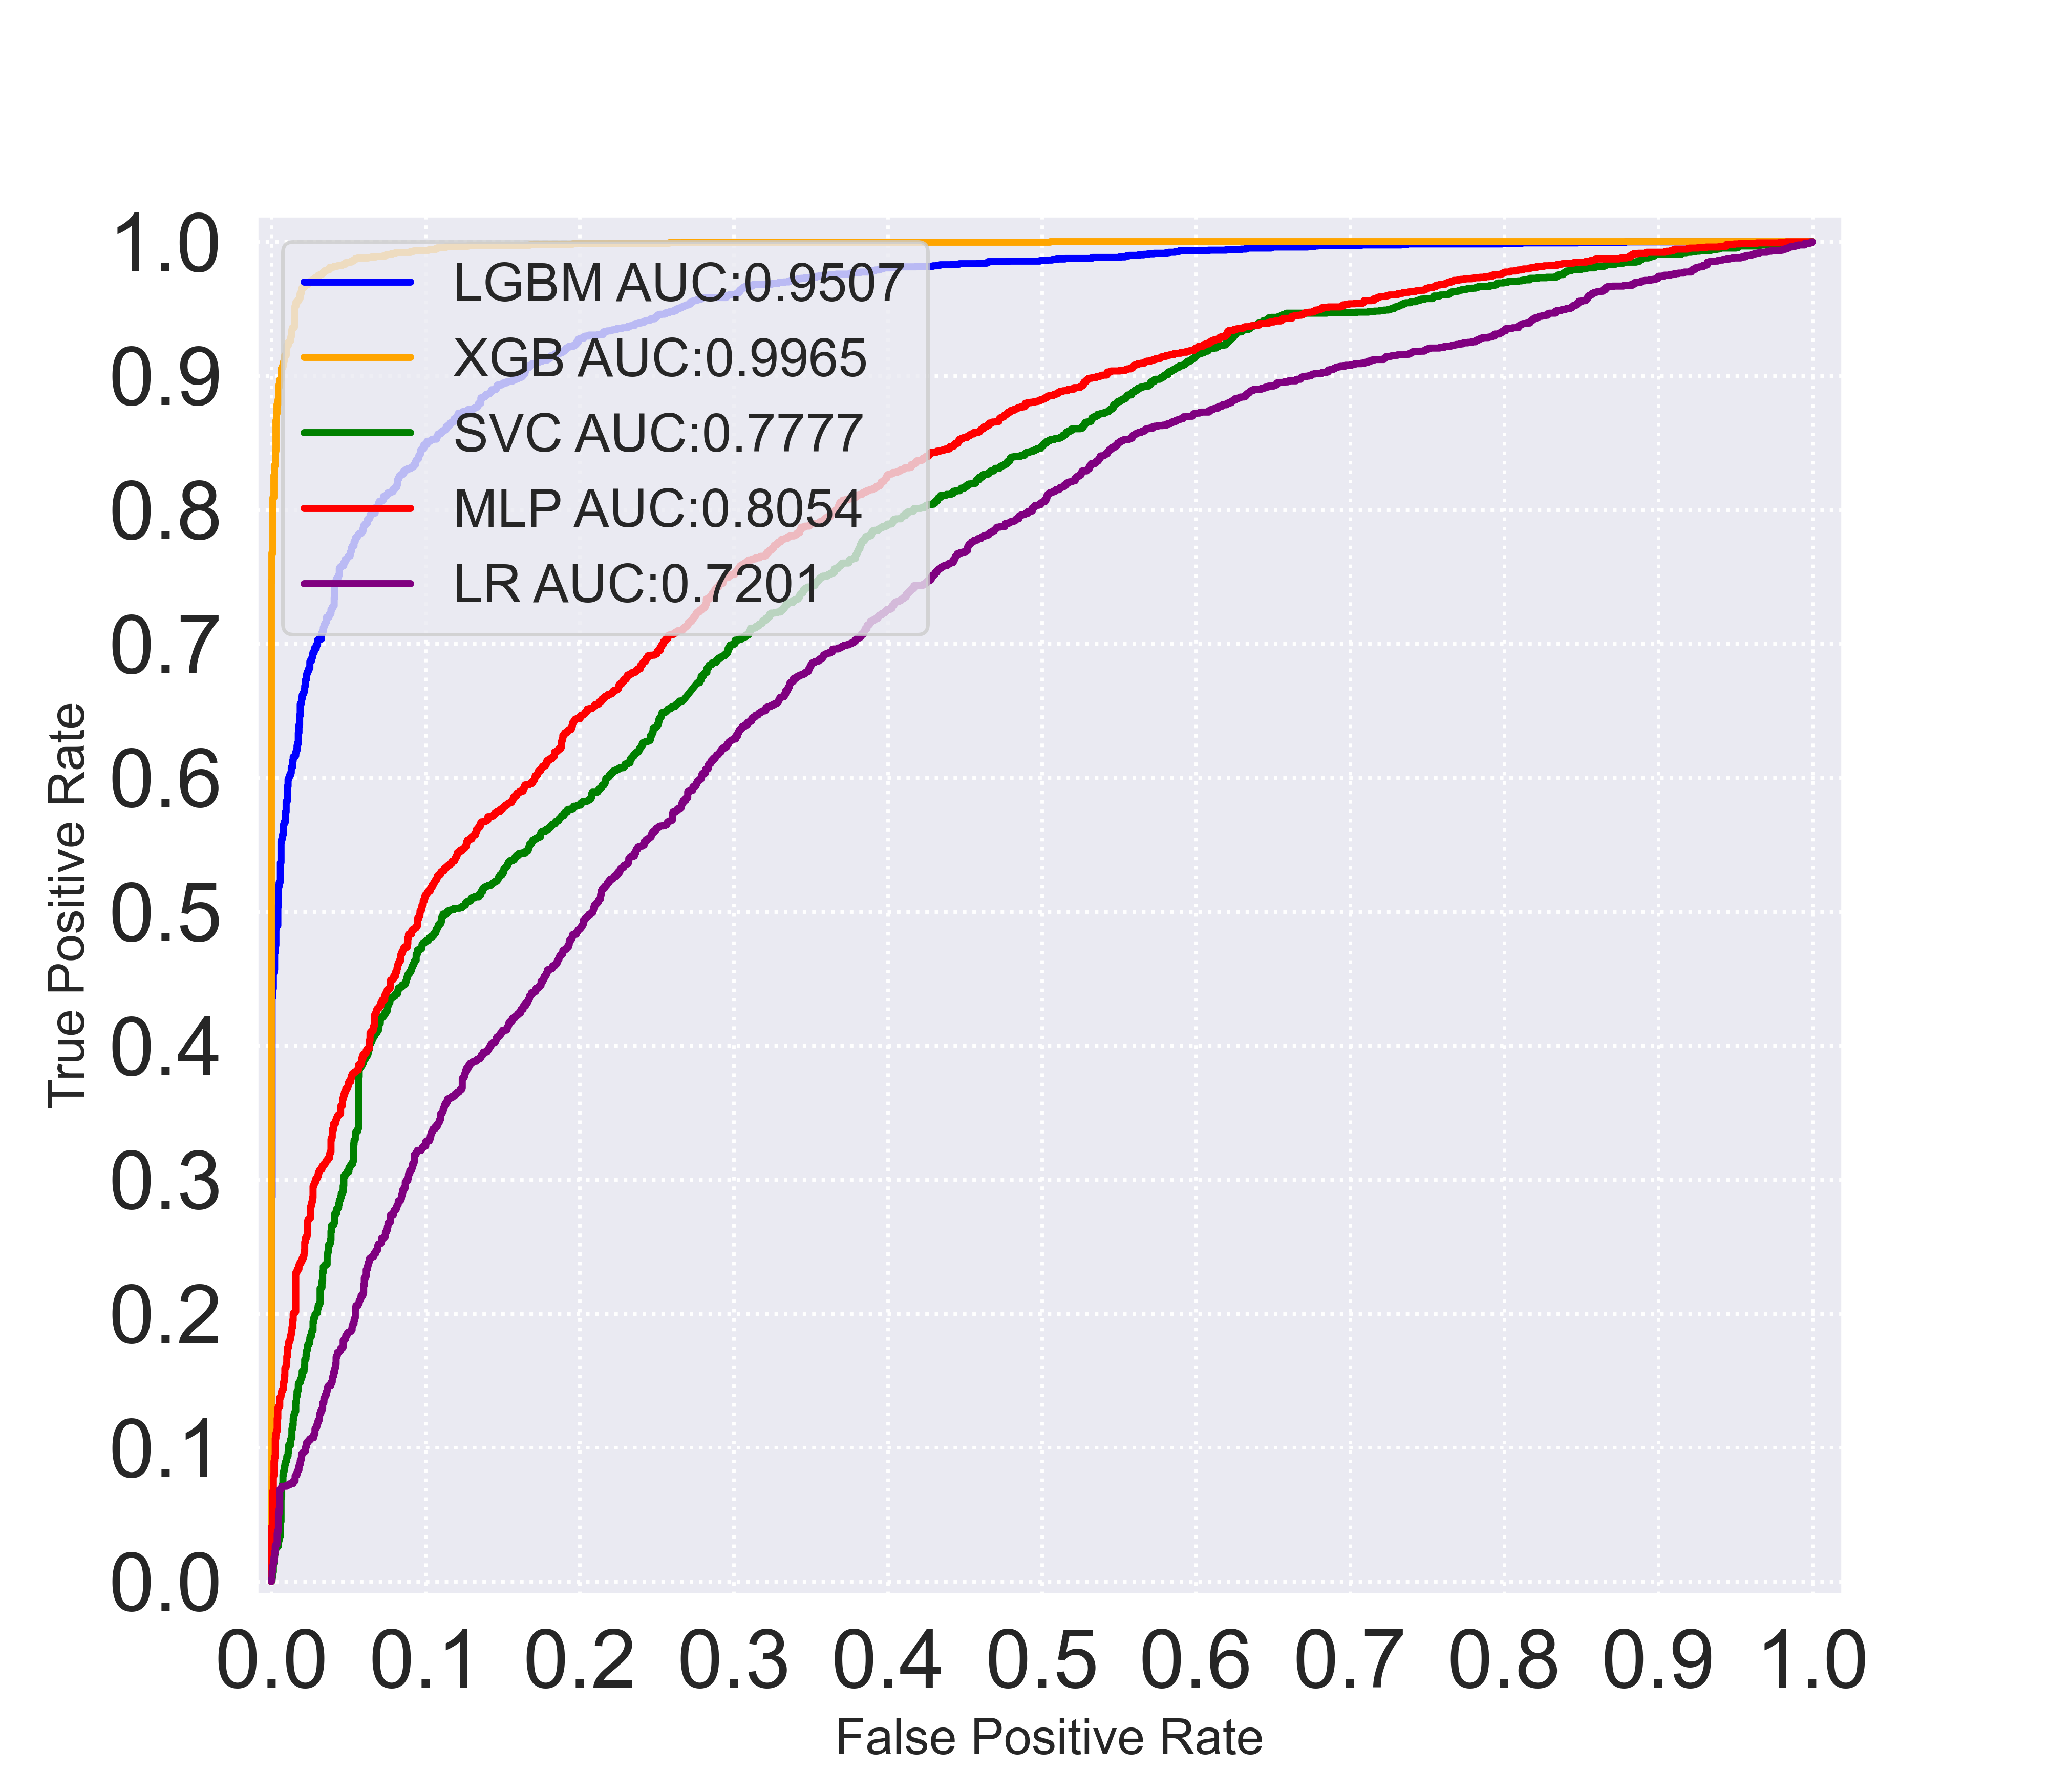
\includegraphics[width=\linewidth]{task1_image\roc_auc(train(before_sampling)).png} % Replace 'figure2' with the filename of your second figure
          \caption{roc_auc_train}
          \label{fig:roc_train}
      \end{subfigure}
      \caption{Overall caption for the figures}
      \label{fig:overall}
\end{figure}
\bibliographystyle{alpha}
\bibliography{sample}

\end{document}